\documentclass[11pt]{aghdpl}
\usepackage[polish]{babel}
\usepackage[utf8]{inputenc}
\usepackage{enumitem}
\usepackage{listings}
\usepackage{graphicx}
\usepackage{subcaption}
\usepackage{capt-of}
\usepackage{multirow}
\usepackage{xcolor,colortbl}
\usepackage{longtable}
\usepackage{pdflscape}
\usepackage{array}
\usepackage{url}
\usepackage{varwidth}
\usepackage{hyperref}

\hypersetup{
    colorlinks,
    citecolor=black,
    filecolor=black,
    linkcolor=black,
    urlcolor=black
}

\definecolor{Gray}{gray}{0.75}
\definecolor{LightGray}{gray}{0.90}
\setitemize{itemsep=3pt,topsep=3pt,parsep=3pt,partopsep=3pt}
% Command	What it does
% \parskip
% Space between paragraphs outside of a list, and part of the space between a non-list paragraph and a list item.
% \topsep
% Extra space added to \parskip before the first and after the last item.
% \parsep
% Paragraph separation within a single item.
% \itemsep
% Extra inter-item spacing added to \parsep.
% \partopsep
% This is added to the top and/or bottom of the list if and only if there's a blank line above or below the first or last item. Leave this alone unless blank lines become a problem.
% nic nie chce dzialać
\let\oldenumerate\enumerate
\renewcommand{\enumerate}{
  \oldenumerate
  \setlength{\itemsep}{0pt}
  \setlength{\topsep}{0pt}
  \setlength{\parsep}{0pt}
  \setlength{\partopsep}{0pt}
}
\setlist[enumerate]{leftmargin=14mm}
\def \longauthor{Krzysztof Spytkowski, Magdalena Warzecha}
\author{Wojciech Kasperek, Agnieszka Maksylewicz,}
\shortauthor{W. Kasperek, A. Maksylewicz, K. Spytkowski, M. Warzecha}

\titlePL{Implementacja mechanizmu server-push z wykorzystaniem techniki piggy-back w technologii EJB3}
\titleEN{}

\shorttitlePL{Implementacja mechanizmu server-push z wykorzystaniem techniki piggy-back w technologii EJB3}
\shorttitleEN{}

\thesistype{}

\supervisor{dr Rafał Mrówka}

\degreeprogramme{Informatyka}

\subject{Wprowadzenie do wzorców projektowych}

\date{2014/2015}

\department{Katedra Informatyki Stosowanej}

\faculty{Wydział Elektrotechniki, Automatyki,\protect\\[-1mm] Informatyki i Inżynierii Biomedycznej}
\makeatletter
\newcommand*{\compress}{\@minipagetrue}
\makeatother
\newcommand{\tableEnumerateBegin}{  \noindent\par
\vspace{-\baselineskip}
\compress\begin{enumerate}}
\newcommand{\tableEnumerateEnd}{\end{enumerate}\vspace{-\baselineskip}\vspace{-\baselineskip}}
%---------------------------------------------------------------------------

\begin{document}

\titlepages
\vspace*{-20mm}
\tableofcontents
\clearpage

\chapter{Opis projektu}
Celem projektu jest implementacja mechanizmu server-push przy użyciu techniki piggy-back, wykorzystując odpowiednie wzorce projektowe. Językiem implementacji jest Java EE (EJB3). Na~wstępie warto zapoznać się z~podstawowymi pojęciami dotyczącymi tematu.


\section{Server-push}
Server-push to~mechanizm umożliwiający serwerowi wysyłać dane do~klienta. Należy jednak pamiętać, że~połączenie nawiązywane jest zawsze przez klienta, przez co~nie jest możliwe proste wysyłanie oczekiwanych danych przez serwer bez interakcji z~klientem.

Istnieje klika metod pozwalających osiągnąć zamierzony efekt. Są~to:
\begin{description}
 \item[pooling] odpytywanie serwera w~stałym krótkim interwale czasowym
 \item[piggy-back] opisany w~kolejnej sekcji
 \item[comet] podtrzymywanie zapytania przez serwer do~momentu wygaśnięcia czasowego (timeout) lub do~przybycia oczekiwanych informacji (zwracanych klientowi)
\end{description}


\section{Piggy-back}
Nazwa techniki może zostać przetłumaczona jako~``jazda na~barana''. Może to~sugerować sposób działania metody. 

Klient wysyła zapytanie do~serwera w~celu wykonania pewnej operacji. Serwer ma~za~zadanie wysłać odpowiedź zgodną z~oczekiwaniami klienta. Dodatkowo jednak, jeśli posiada inne informacje do~przekazania klientowi, dołącza je~do odpowiedzi, tworząc \textit{mixed response}.
\begin{center}
 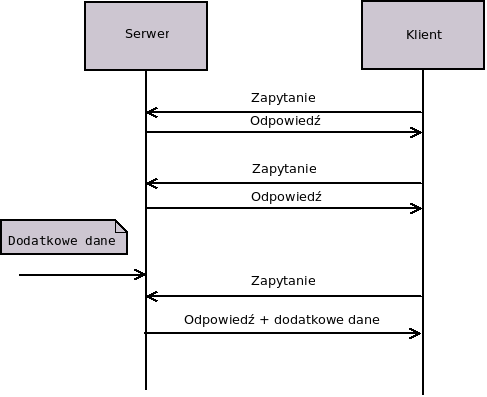
\includegraphics[width=8cm]{piggy}
\end{center}

Jest to~rozwiązanie znacznie wydajniejsze niż~\textit{pooling}, ponieważ nie wykorzystuje dodatkowych zasobów klienta. Ma~jednak swoje wady, ponieważ informacje mogą nigdy nie dotrzeć do~klienta (w~przypadku nie wykonania zapytania) lub też~dotrzeć po~długim czasie. Lepszym rozwiązaniem jest \textit{comet}.

\section{Opis pomysłu}
Stworzona aplikacja to~symulacja działania niezależnych barów (bar plebejski, bar luksusowy) sprzedających napoje alkoholowe. W~każdym barze pracują barmani, których zadaniem jest realizacja zamówień klientów. Wspomniane bary mają w~swojej ofercie kilka typów napojów wyskokowych: piwa (jasne, ciemne) oraz~drinki (Bloody Mary, Pina Colada). W~zależności od~typu baru, barman korzysta z~różnych przepisów przy przygotowywaniu napojów (w~barze plebejskim zamiast części alkoholu dolewa wodę). Może się~jednak zdarzyć, że~w~barze zabraknie jakiegoś składnika koniecznego do~przygotowania napoju. W takim wypadku barman składa zamówienie u~zaprzyjaźnionego dostawcy, który natychmiastowo dostarcza brakujący składnik. Ważnym aspektem jest to, że~każdy barman może wybrać bary, które chciałby ''obserwować'' - wówczas będzie dostawał informacje o~zamówieniach zrealizowanych w~tych barach w~ostatnim czasie. 

\chapter{Architektura}
A tu co?

\chapter{Wzorce projektowe}
W ramach projektu zaimplementowaliśmy następujące wzorce:

\begin{itemize}
 \item 
\end{itemize}


\end{document}